% Generator: hand-authored TikZ schematic traced from the fixed source; triangle proportions are illustrative.
% Source ID: src-dcc6a2c21c7b8e7b8f23f5188f34d7f542f94e40f4219b54cfb85a0d7004bc0f
% PDF SHA-256: 7fc0fd289fc486a0ae1c16a9ab5b4f0561830897df6e8897c50666f03d511913
% PDF page 2; printed page 127; question 19.
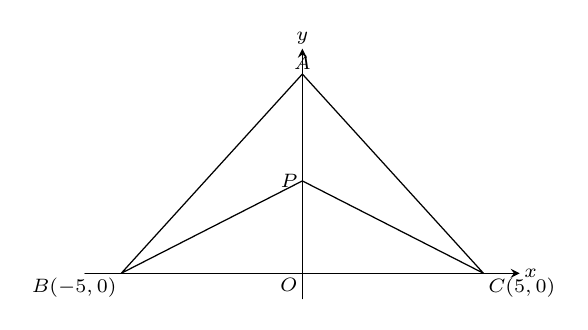
\begin{tikzpicture}[
  x=0.46cm,y=0.46cm,line width=0.45pt,line cap=round,>=stealth,
  every node/.style={font=\scriptsize,inner sep=1.5pt}
]
  \coordinate (O) at (0,0);
  \coordinate (A) at (0,5.5);
  \coordinate (P) at (0,2.55);
  \coordinate (B) at (-5,0);
  \coordinate (C) at (5,0);

  \draw[->] (-6.0,0)--(6.0,0) node[right] {$x$};
  \draw[->] (0,-0.7)--(0,6.2) node[above] {$y$};
  \draw (A)--(B) (A)--(C) (P)--(B) (P)--(C);

  \node[above] at (A) {$A$};
  \node[below left] at (B) {$B(-5,0)$};
  \node[below right] at (C) {$C(5,0)$};
  \node[below left] at (O) {$O$};
  \node[left] at (P) {$P$};
\end{tikzpicture}
